%!TEX root = ../main.tex

\chapter{Monitoring}
\label{ch:monitoring}

The section will detail \cref{sec:verification_techniques} \reftextfaraway{sec:verification_techniques}, where monitoring as a runtime verification technique was introduced.

As previously stated, monitoring is a runtime verification method, when the system is checked against a reduced model of the system. The monitor model contains error states, which represent non specified behavior. This reduced model easier to developed usually by model based technologies e.g.\ automaton, and checked by formal verification methods.

\section{Agent based monitoring}

The monitor itself must be notified about the current state the monitored component. To notify the monitor about this states, the monitored component contains a component called \emph{agent}. The agent is responsible to notify the monitor\,--if it's remote or local--\,about the state of the monitored component.  \cref{fig:agent_based_monitoring} depict a base component diagram of an agent based monitoring system.

\subsection{Agent communication}

The \cref{fig:agent_based_monitoring} depicting the communication between elements bidirectional. This direction of the way of communication between the agent, and monitor can be divided into two groups:
\begin{itemize}
	\item \emph{Push:} The agent sends the state changes to the monitor.
	\item \emph{Pull:} The monitor queries the agent to get the current state the agent is in.
\end{itemize}

This methodology is the same for communication between monitors, and external systems may interested in the state of the monitor.

\begin{figure}[h]
	\centering
	\begin{tikzpicture}[
		every node/.style = {
				align=center,
				anchor=north west
			}
		]

		\node[squarednode] (MC) at (4,0) [text width=4cm, minimum height=2.5cm] {}
			node [below = 0.15cm of MC.north] {Monitored component}
			node [squarednode] [above = 0.25cm of MC.south, text width=3cm] (EA) {Embedded\\agent};
		\node[right = 3cm of MC, squarednode, minimum height=2.5cm] (M) [] {Monitor};

		\draw[thick,<->] (EA.east) -- (M.west |- EA.east) node [pos=0.6, below] {Signals};
		\draw[thick,<->] ([yshift=.5cm]M.west) -- ([yshift=.5cm]MC.east) node [midway, above] {Error states};

	\end{tikzpicture}

	\caption{Agent based monitoring schematic}
\label{fig:agent_based_monitoring}
\end{figure}

\section{Monitor automata}

As mentioned before, a practical formalism for monitoring purposes is the automaton. Automaton are really flexible constructions, and possibile usages can vary from simple event automaton to parametrized, timed automaton. Other factors, as deterministic, and non-deterministic automaton must be dealt with in the generation process.

\section{Example of monitor automata}

To illustrate how a reduced model can help the monitoring of a complex system, let's review a simple monitor automata (\cref{sec:automata}) depicted in \cref{fig:example_monitoring_basics}.

The example monitors a network communication. The monitored component sends a request\,--thus entering state \emph{2}--\,and waits for response. If the response arrived before the \SI{10}{\ms} elapsed, the automata returns to state \emph{1}. If the wait for the response exceeds the \SI{10}{ms} time window, the automata enters into the \emph{ERROR} state.

\begin{figure}[h]
	\centering
	\begin{tikzpicture} [
			auto,
			every path/.style = {
				thick,
				->
			},
		]
		\node[circle, very thick, draw=black, minimum size=15mm] (A) [] {1};
		\node[circle, very thick, draw=black, minimum size=15mm] (B) [right = 2.5cm of A] {2};
		\node[circle, very thick, draw=black, minimum size=15mm, fill=black!10] (C) [right = 3cm of B] {ERROR};

		\draw (A) ++(-2, 1) -- (A);
		\draw (A) edge [bend left]
			node [sloped, midway, above] {request sent} (B);
		\draw (B) edge [bend left]
			node [sloped, midway, below] {response received} (A);
		\draw (B) edge [bend left]
			node [sloped, midway, above] {after \SI{10}{\ms}} (C);

	\end{tikzpicture}
	\caption{Simple monitoring example}
\label{fig:example_monitoring_basics}
\end{figure}

\section{\viatrac{}}

The \viatrac{} is a complex event processing frameworks, based on Eclipse technologies such EMF, and \viatraq{}. \viatrac{} uses regular expression to define patterns. With regular expression, the developer gets an expressive formalism. Existing knowledge can be used while using regular expressions because of it's widespread usage in text matching. The \viatrac{} formalism in most of the part follows the syntax of text based regex matching.

\subsection{\viatrac{} regex formalism}
\label{sec:viatra_regex}

This section briefly introduce the elements of the formal language, which is developed as a work of \cite{laszlo}. An expression may consists of the elements denoted in \cref{fig:regex}.
\begin{figure}
	\centering
	\caption{Code size in bytes with respect to compiler optimization levels, and alphabet size}
	\begin{tabular}{l l l}
		\toprule
		Regex & Explanation & Example \\
		\midrule
		A & Matching event A & A \\
		A B & Matching event A and B, in strict order & AB \\
		A \& B & Matching event A and B, non-ordered  & BA \\
		A (A \& B) & Grouping expressions & AAB or ABA \\
		A+ & 1 or more captured expression & A\ldots \\
		A* & 0 or more captured expression & AAAA\ldots \\
		{A}<x> & The expression should match in x time units & \\
		\bottomrule
	\end{tabular}
	\label{fig:regex}
\end{figure}

\subsection{\viatrac{} automaton}
\label{sec:metamodel}

This section will introduce the automaton metamodel of the \viatrac{}. This metamodel is a very fundamental to the code generation process, because compiled regular expressions are compiled as an instance model of this metamodel.

\subsubsection{Basic automaton partial model}

\begin{figure}[h]
	\centering
	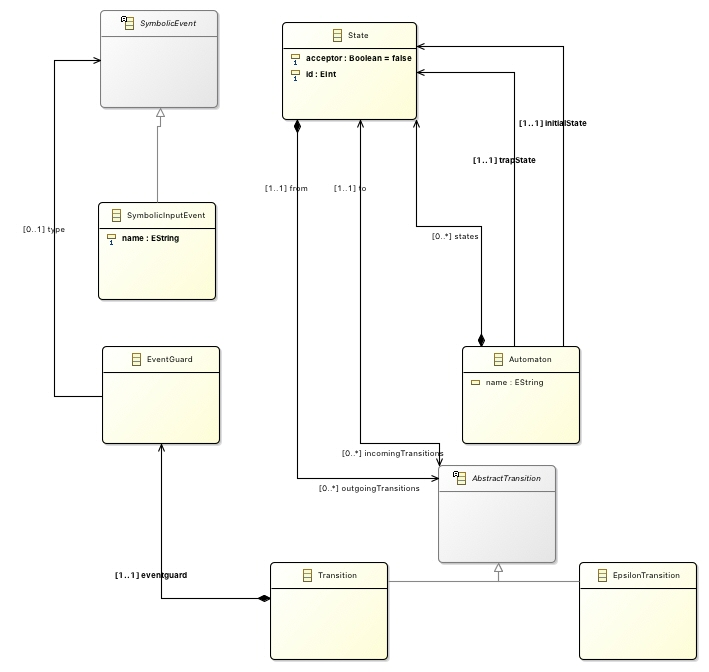
\includegraphics[width = \textwidth]{include/figures/basic_automaton}
	\caption{The \emf{} metamodel of the \viatrac{} automata}
\label{fig:basic_automaton}
\end{figure}

\cref{fig:basic_automaton} illustrate the very core of this metamodel. This automaton model is rather extensible in a way timed or parametrized attachments can be used when creating the instance model, but they not necessarily needed. What \cref{fig:basic_automaton} depict is a basic automaton.
\begin{itemize}
	\item Automaton classes contains states, and have reference to the initial state of the automaton.
	\item States are unique, identified by an id. Each state can be an acceptor state, meaning if a word which was processed by the automaton reaches an acceptor state becomes an accepted word of the automaton. States can contain outgoing transitions, and have reference of transitions, which point to them.
	\item Transitions interconnect states. The transition have an incoming, and outgoing state reference. Transitions can have guards, which can be symbolic, and later on, related to timing.
	\item EpsilonTransition is a special kind of transition, which is used in the compilation process. A non-deterministic automaton might contain epsilon transitions, but the code-generation this thesis implements works on a deterministic automaton, therefore this kind of transition will not be present in the instance models.
\end{itemize}

\subsubsection{Timing additions to the automaton model}

\begin{figure}[h]
	\centering
	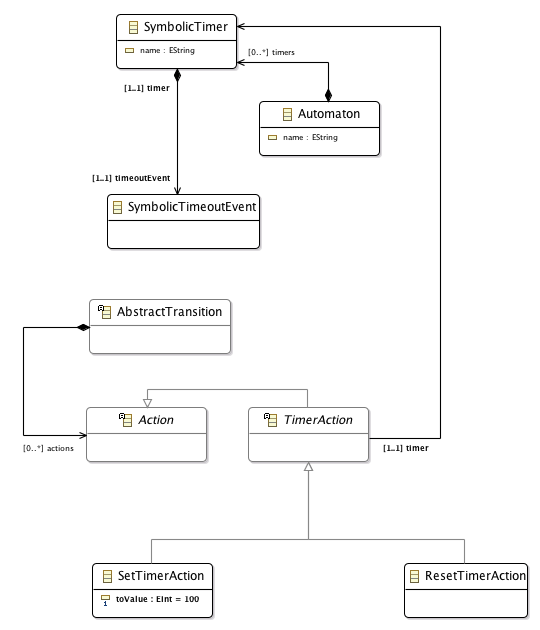
\includegraphics[width = \textwidth]{include/figures/timing_diagram}
	\caption{The \emf{} metamodel of the \viatrac{} timing additions}
\label{fig:timed_automaton}
\end{figure}

Timing metamodel additions are extensions to the basic automaton metamodel, to be usable with temporal expressions.
\begin{itemize}
	\item automaton can have symbolic timers, identified by name.
	\item Set action can set the time values. After the timers are set to a value, the timer implicitly activates, and start counting down.
	\item Reset action can stop the timer counting down, thus prevent it to timeout. On the other hand, the timer value is set to the specified value it was last assigned of.
	\item Set and reset actions are the two key actions, which can be used to implement timing automaton.
	\item Symbolic timer can raise timeout event, which indicates that the timer run out of the specific time value it was set to.
\end{itemize}

With this metamodel, one can compile an instance model representing the monitoring automata.

Because it's a metamodel, it does not contain any information about the behavior of the automaton. The execution of a metamodel is up to the developer of the system. A generic approach is to write a simulator.

The current \viatrac{} automaton utilizes a simulation technique. By writing \viatraq{} patterns, the simulator can work on any valid metamodel, providing a generic execution backend for the formalism. Simulation have disadvantages, which is more severe in lower end devices. The resource need of a simulation is complex. In this case, the \viatraq{} engine post a serious memory pressure, because it's caching mechanism.

On the other hand, code generation can be used. In this case this thesis utilizes code generation to generate source code to a specific automaton, thus reducing the complexity of a generic execution. \cref{ch:codegen} will introduce this techniques.
